\documentclass[t]{beamer}
%\usetheme{amcg}
\usetheme{iclpt}

\usepackage{color,listings}
\usepackage{pstricks, pst-node}
\usepackage{pgfpages,xspace,array}

\newcommand{\doc}[1]{\psshadowbox[framearc=0]{#1}}
\newcommand{\program}[1]{\psframebox[framearc=.2]{#1}}

\usepackage{graphicx,stmaryrd,cancel}
\usepackage{bibentry}
\usepackage{hyperref}
\usepackage{amscd}
\usepackage{booktabs}
\bibliographystyle{elsarticle-harv}

\lstset{frame=single}

\expandafter\ifx\csname natexlab\endcsname\relax\def\natexlab#1{#1}\fi
\expandafter\ifx\csname url\endcsname\relax
  \def\url#1{\texttt{#1}}\fi
\expandafter\ifx\csname urlprefix\endcsname\relax\def\urlprefix{URL }\fi

\definecolor{icdarkblue}{RGB}{23,18,134}
\definecolor{icdarkgreen}{RGB}{0,130,0}

%\setbeameroption{show notes on second screen}

\author[David A. Ham]{Dr David~A.~Ham} 
\date{24 May 2013}

\title{Introduction to software configuration management}
                  
\institute[Imperial College London]{
  Department of Computing, Imperial College London\\
  Grantham Institute for Climate Change, Imperial College London
david.ham@imperial.ac.uk}

\begin{document}
\nobibliography{bibliography}

\begin{frame}{}
  \vfill{}

  \centering

  \Large\color{icdarkblue}\inserttitle\\
  %\normalsize\insertsubtitle\\[3ex]
  \small\color{black}\insertauthor\\[3ex]
  \footnotesize\insertinstitute

  \vfill{}

\end{frame}

\begin{frame}{Software configuration management topics}

  \begin{itemize}
  \item Version control
  \item Building on different platforms
  \item Testing
  \end{itemize}
  
\end{frame}

\begin{frame}{Version control: getting the source right}
  
  \begin{itemize}
  \item ``Nobody knows which version of the code was used to create the
    plots in the paper, and now the reviewers want more runs!''
    \pause
  \item ``Alice has a slope limiter in her version of foo.cpp, and Bob's version has a
    turbulence model, but I want a slope limiter \emph{and} a turbulence
    model.''
    \pause
  \item ``I think Charlie had that feature in a version on his laptop
    somewhere, but he's working for a bank now.'' 
    \pause
  \item \Huge\hspace{1.5em}``This used to work!''
  \end{itemize}

\end{frame}

\begin{frame}{The core idea behind a version control system}

  \centering
  
  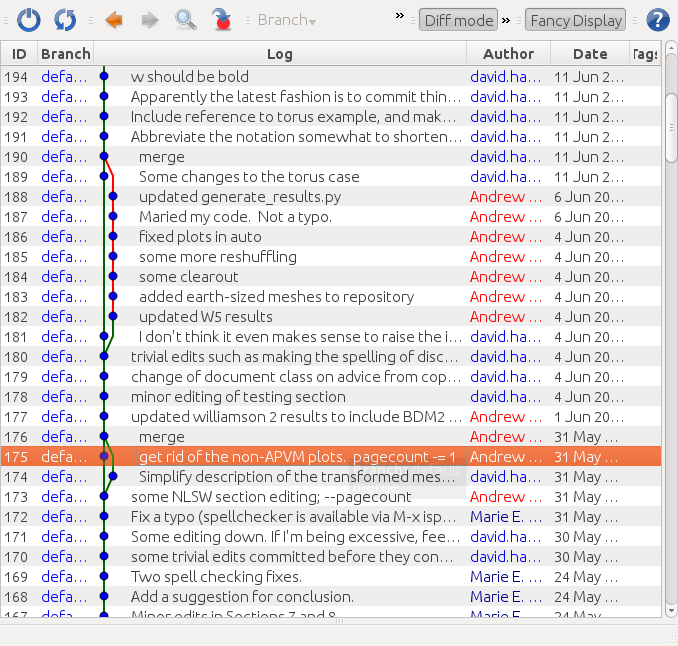
\includegraphics[height=.8\textheight]{mercurial_paper.png}

  A simple example, several co-authors work on the same paper. 
  
\end{frame}

\begin{frame}{The core ideas behind a version control system}
  
  \begin{itemize}
  \item Keeping each version of your files as they develop is partly automated.
  \item You can always get back to any version of your files.
  \item It's very easy to see the differences between different versions of files.
  \item The conflicts caused by multiple people editing the same files are minimised.
  \end{itemize}

\end{frame}

\input{vcs.tex}

\begin{frame}{Branching}
  
  So far so good, but what if you want to make a more substantial change
  which should be spread over many commits?
  
\end{frame}

\input{branching.tex}

\begin{frame}{Merging back}

  So now we know how to work on a feature branch, how do we get our changes
  back into the trunk?
  
\end{frame}

\input{branch_merging.tex}

\begin{frame}{Feature branches are a Good Thing}

  \begin{itemize}
  \item Keep the trunk in working order.
  \item Different developers can work independently.
  \item Encourages frequent commits.
  \item Facilitates code review (we'll come back to this).
  \end{itemize}
  
\end{frame}

\input{dvcs.tex}

\begin{frame}{Distributed version control systems}
  
  Advantages:
  \begin{itemize}
  \item Most operations are local and so fast. These also work offline.
  \item More complex workflows involving lots of peers are facilitated.
  \item Merging is faster and less trouble than with centralised systems.
  \end{itemize}

  (Alleged) drawbacks:
  \begin{itemize}
  \item Simple tasks can require more commands than in a centralised system.
  \item Valuable code is not automatically stored somewhere safe.
  \end{itemize}

\end{frame}

\begin{frame}{Common version control systems}
  
  Centralised:
  \begin{description}
  \item[CVS] Used to be very common, now rather old-fashioned and hard to
    work with. Avoid if possible
  \item[SVN] Very widely used.
  \end{description}

  Distributed:
  \begin{description}
  \item[Git] Probably the most commonly used modern system.
  \item[Mercurial (hg)] Competitor to git but with syntax more similar to SVN.
  \item[Bazaar (bzr)] Fairly similar to hg. Extensively used by software related to Ubuntu Linux,
    but no longer actively developed. 
  \end{description}

\end{frame}

\begin{frame}{Version control system hosting}

  \small
  Various companies offer the service of hosting version control
  repositories via web interfaces. These are often free if your project is
  open source and/or you are affiliated with a university.
  \vspace{1ex}
  
  The services may also include outher software development tools such as
  bug trackers, documentation hosting, fora etc.
  \vspace{1ex}  

  \begin{centering}
  \framebox{
  \begin{tabular}{l|l}
    Github & git \\
    Bitbucket & git and hg \\
    Launchpad & bzr\\
    Sourceforge & git, hg and svn 
  \end{tabular}}    

  \end{centering}
  \vspace{1ex}  

  A particularly useful feature of Bitbucket is that it offers unlimited
  private repositories to university users.
  \vspace{1ex}  
  
  Many departments also offer repository hosting to staff and students.

\end{frame}

\begin{frame}{Code review}
  
  Having other people read your code is one of the best ways of ensuring
  quality. Version control hosting sites often support this via a web
  interface for \emph{pull requests} or \emph{merge requests}.

\end{frame}

\input{pull_request}
\input{pull_request_2}

% \begin{frame}{Simulation workflow management}

%   Find that cool thing Florian showed me.
  
% \end{frame}

\begin{frame}{Build configuration}

  How do you make your software work on different machines, with different
  compilers, different library locations\ldots
  
\end{frame}

\begin{frame}[fragile]{In the beginning there was make}
  We can write a Makefile containing rules for compiling our code:
  \begin{lstlisting}[language=make]
foo: foo.c foo.h bar.o 
    gcc -o foo foo.c foo.o

bar.o: bar.c bar.h
    gcc -c bar.c
  \end{lstlisting}

  Now typing:
  \begin{lstlisting}[language=bash]
>> make foo
  \end{lstlisting}
  will cause exactly those complations which are needed in order to build foo.
  
\end{frame}

%Show some make commands.
\begin{frame}{In the beginning there was make}
  With make you can:
  \begin{itemize}
  \item specify that certain files are built from other files.
  \item let make figure out which files have changed and what order to build in.
  \item make basic choices about things like which compiler to use by
    setting environment variables.
  \end{itemize}
  but make cannot:
  \begin{itemize}
  \item automatically find the right libraries for you.
  \item specify different compilation configurations for different environments.
  \item easily turn on and off additional features.
  \item help make configuration compiler-independent.
  \end{itemize}
\end{frame}

\begin{frame}{Configuration generation tools}

  \begin{itemize}
  \item Typically use a scripting language to write a program which knows
    how to build a project.
  \item Use a variety of scripting languages.
  \item Typically provide large libraries of functionality for common tasks
    (e.g. finding Python, or common libraries).
  \item May build the project directly (e.g. SCons), or write Makefiles which
    build the project (e.g. automake/autoconf CMake).
  \item Typically honour conventional environment variables (e.g. CC,
    CFLAGS, PETSC_DIR) and so ``play nice'' alongside system adminstration
    tools like environment modules.
  \end{itemize}
  
\end{frame}


\end{document}
